\chapter{Especificación de requisitos}

\noindent\fbox{
	\parbox{\textwidth}{
		En esta sección se tratarán de recoger todos los detalles que definan y limiten el funcionamiento de la aplicación.
	}
}

\section{Personas: ¿Quienes lo podrían usar?}

Para poder hacernos una idea de los posibles usos del Asistente de Voz se ha decidido crear una serie de personas ficticias que, para poder facilitar algún aspecto de su vida, puedan usar este producto.

En las tablas de las siguientes páginas, podemos encontrar una información somera de estas personas:

\begin{itemize}
	\item \textbf{Irene Fernández}, una estudiante de Bachiller en una fase de exámenes finales antes de la Selectividad, donde acaba por planear su estudio y el tiempo que le queda para poder acabar el curso y entrar a su carrera vocacional en la Universidad.
	
	\item \textbf{Javier Pedrosa}, un funcionario que recientemente perdió parte de la visión por un accidente, entrando en una nueva fase de su vida donde la tecnología le ayuda a poder tener cierta autonomía.
\end{itemize}

Si bien estos casos pueden necesitar soluciones concretas, el objetivo con este proyecto es que si alguna función no se pudiera realizar en este momento, gracias a la modularidad cualquiera pudiera integrar alguna utilidad para suplir esas demandas.

\newpage

\begin{table}[H]
	\centering
	\begin{tabular}{|l|l|l|} 
		\hline
		Nombre       & Irene Fernández & \multirow{4}{*}{
			\begin{minipage}[t]{0.4\textwidth}
				\begin{center}
					 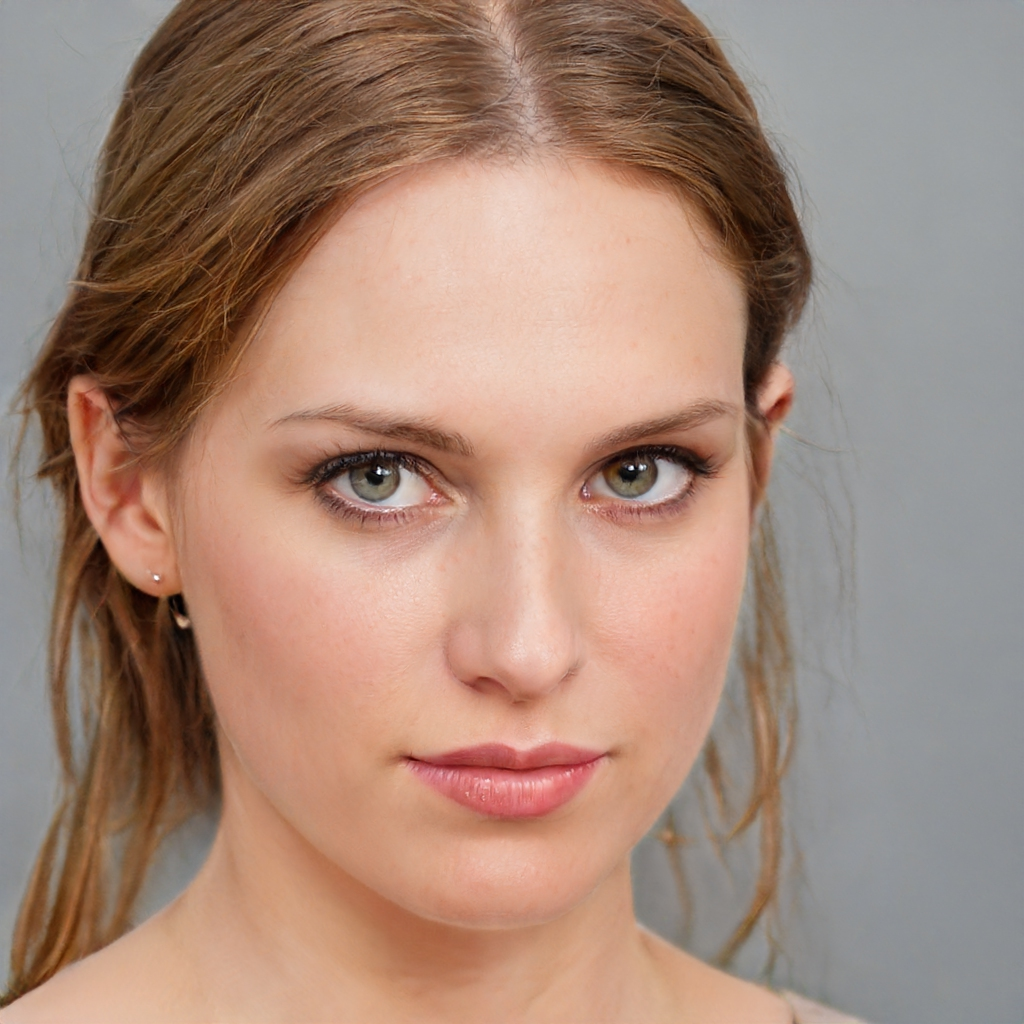
\includegraphics[height=3cm]{imagenes/Persona1.jpg}
				\end{center}
			\end{minipage}
			}                 \\ [2ex]
		\cline{1-2}
		Edad         & 19 &                                   \\ [2ex] 
		\cline{1-2}
		Género         & Femenino &                                   \\ [2ex]
		\cline{1-2}
		Educación    & Bachillerato Científico-Sanitario &                                   \\ [2ex] 
		\hline
		\multicolumn{3}{|l|}{\cellcolor{lightblue}\textbf{Contexto de uso}}               \\ 
		\hline
		Cuándo       & \multicolumn{2}{l|}{Tras las clases, antes de ponerse a estudiar}                \\ 
		\hline
		Dónde        & \multicolumn{2}{l|}{Ordenador portátil}                \\ 
		\hline
		\multicolumn{3}{|l|}{\cellcolor{lightblue}\textbf{Misión}}                        \\ 
		\hline
		Objetivo     & \multicolumn{2}{l|}{Tener una ayuda en el estudio}                \\ 
		\hline
		Expectativas & \multicolumn{2}{l|}{
			\begin{minipage} [t] {0.7\textwidth}
				\begin{itemize}
					\item Permitir hacer control del tiempo a través de contadores regresivos
					\item Permitir realizar cálculos sencillos
					\item Recordar tareas pendientes
				\end{itemize}
			\end{minipage}
		}                \\ 
		\hline
		\multicolumn{3}{|l|}{\cellcolor{lightblue}\textbf{Motivación}}                   \\ 
		\hline
		Urgencia     & \multicolumn{2}{l|}{
			\begin{minipage}[t]{0.7\textwidth}
				No le sería de mucha urgencia, ya que puede usar otras herramientas (Reloj/Cronómetro, Agenda, Calculadora...)
			\end{minipage}
		}                \\ 
		\hline
		Deseo        & \multicolumn{2}{l|}{
			\begin{minipage}[t]{0.7\textwidth}
				Siente que llevar tantas cosas para poder organizar su vida puede ser un tanto engorro, y centralizar sus utilidades en algo que lleve consigo como su portátil o su teléfono podría ahorrarle tantas molestias.
			\end{minipage}
		}                \\ 
		\hline
		\multicolumn{3}{|l|}{\cellcolor{lightblue}\textbf{Actitud ante la tecnología}}    \\ 
		\hline
		\multicolumn{3}{|l|}{
			\begin{minipage}[t]{\textwidth}
				Sabe manejar el ordenador en programas de ofimática como Word y Powerpoint; usa el navegador constantemente para ver sus redes sociales y buscar lo que necesite
			\end{minipage}
		}                              \\
		\hline
	\end{tabular}
	\caption[Ficha Persona 1]{Ficha de la Persona 1 (Irene Fernández). Imagen extraída de \cite{thispersondoesnotexist}}
\end{table}

\newpage

\begin{table}[H]
	\centering
	\begin{tabular}{|l|l|l|} 
		\hline
		Nombre       & Javier Pedrosa & \multirow{4}{*}{
			\begin{minipage}[t]{0.4\textwidth}
				\begin{center}
					
\includegraphics[height=3cm]{imagenes/Persona2.jpg}
				\end{center}
			\end{minipage}
		}                 \\ [2ex]
		\cline{1-2}
		Edad         & 46 &                                   \\ [2ex] 
		\cline{1-2}
		Género         & Masculino &                                   \\ [2ex]
		\cline{1-2}
		Profesión    & 
			\begin{minipage}[t]{0.3 \textwidth}
				Funcionario
			\end{minipage}
		 &                                   \\ [2ex] 
		\hline
		\multicolumn{3}{|l|}{\cellcolor{lightblue}\textbf{Contexto de uso}}               \\ 
		\hline
		Cuándo       & \multicolumn{2}{l|}{Al llegar a casa}                \\ 
		\hline
		Dónde        & \multicolumn{2}{l|}{Ordenador portátil y/o aparato dedicado}                \\ 
		\hline
		\multicolumn{3}{|l|}{\cellcolor{lightblue}\textbf{Misión}}                        \\ 
		\hline
		Objetivo     & \multicolumn{2}{l|}{Poder disfrutar de cierta independencia}                \\ 
		\hline
		Expectativas & \multicolumn{2}{l|}{
			\begin{minipage} [t] {0.7\textwidth}
				\begin{itemize}
					\item Permitir escuchar alguna información proveniente de Internet (Noticias, Tiempo...)
					\item Escuchar música, podcasts...
				\end{itemize}
			\end{minipage}
		}                \\ 
		\hline
		\multicolumn{3}{|l|}{\cellcolor{lightblue}\textbf{Motivación}}                   \\ 
		\hline
		Urgencia     & \multicolumn{2}{l|}{
			\begin{minipage}[t]{0.7\textwidth}
				No le sería de mucha urgencia, pero le encantaría tenerlo cuanto antes
			\end{minipage}
		}                \\ 
		\hline
		Deseo        & \multicolumn{2}{l|}{
			\begin{minipage}[t]{0.7\textwidth}
				Desde que perdió parcialmente la visión, no ha podido volver a dedicarse a pasiones como la literatura de forma fácil (por ejemplo, teniendo que esperar bastante tiempo para obtener audiolibros o libros adaptados a braille) o informarse en cualquier momento sin tener que pasar por el ordenador adaptado.
			\end{minipage}
		}                \\ 
		\hline
		\multicolumn{3}{|l|}{\cellcolor{lightblue}\textbf{Actitud ante la tecnología}}    \\ 
		\hline
		\multicolumn{3}{|l|}{
			\begin{minipage}[t]{\textwidth}
				Apenas usa el ordenador para alguna que otra gestión del trabajo.
			\end{minipage}
		}                              \\
		\hline
	\end{tabular}
	\caption[Ficha Persona 2]{Ficha de la Persona 2 (Javier Pedrosa). Imagen extraída de \cite{thispersondoesnotexist}}
\end{table}

\newpage

\section{Casos de uso: ¿Qué podrían hacer?}

Una vez pensado en posibles perfiles de uso, podríamos preguntarnos por alguna incidencia que pudiera solucionarse o facilitarse gracias al sistema resultante.

\subsection{Caso 1: Irene y el calendario de exámenes}

Para nuestra primera persona podemos tener el siguiente caso:

`` \textit{5 de Abril de 2022. Se acerca la época de exámenes finales y poco a poco Irene va teniendo las fechas de estos. Viendo que es el momento de ponerse a prepararlos, apunta todos en su agenda, pero como en esta tiene además las tareas que ha de realizar, decide apuntar esos exámenes en el teléfono y en una hoja de calendario que tendrá que imprimir en la librería de al lado de su casa.}

\textit{Al llegar a casa, coge el teléfono y los va anotando. Además, descarga un PDF con el calendario del mes y llega a la tienda para imprimirlos. Al volver, también los anota, aunque con algo de prisa para ponerse a hacer las tareas que tenía que terminar para mañana. En el descuido los deja en un estante mal colocados y se caen al suelo mojado tras fregar la habitación, dejando la tinta borrosa.}

\textit{Al verlo, Irene se enfada un tanto por tener que volver a hacer el calendario.} ''

\textbf{¿Cómo se podría entonces solucionar este problema?} Podríamos aplicar el Asistente a través de una conversación donde se podría comunicar las fechas con tal de crear recordatorios o consultar a través de la voz si tiene algún evento en los próximos días.

Podríamos así tener una conversación para cada examen que quisiera introducir similar a:

\textit{
	\begin{itemize}
		\item \textbf{Irene}: Recuérdame que tengo examen de Historia de España el 22 de Abril.
		\item \textbf{Bot}: De acuerdo, el 22 de Abril te recordaré ``Examen de Historia de España''
	\end{itemize}
}

\subsection{Caso 2: Irene y la técnica Pomodoro}

Continuando con nuestra primera persona, podríamos darnos con otro caso en el que integrar el software podría servirle de ayuda.

`` \textit{15 de Abril de 2022. Una semana para el examen de Historia de España. Irene va a su cuarto con su reloj y prepara un temporizador de 25 minutos.}

\textit{Mientras estudia, se queda tan centrada que pasa al tiempo de descanso sin notar que el reloj ha vibrado. Cuando mira el reloj, se había pasado media hora más, así que se piensa hacer los 5 minutos de descanso en ese momento antes de activar el temporizador otra vez. Pero en ese caso tenía que estar pendiente del tiempo para no pasarse.} 

\textit{El día acabó siendo bastante fructífero y había preparado sus apuntes para poder seguir estudiando al día siguiente, pero fue un tanto molesto para ella ya que estar pendiente del reloj era un poco engorroso.}''

\textbf{¿Cómo se podría entonces solucionar este problema?} Podríamos aplicar el Asistente a través de dos cuentas atrás, una para la parte de estudio y otra para la parte de descanso, y pedir verbalmente que lo repita X veces, o que simplemente a través de pedir que ponga un contador Pomodoro se genere una conversación para configurar los tiempos y activarse automáticamente.

Podríamos así tener dos estilos de conversación:

La primera opción, que se repitiría tres veces:
\textit{
	\begin{itemize}
		\item \textbf{Irene}: Bot, ponme un contador de 25 minutos
		\item \textbf{Bot}: Contador en marcha
		\item \textbf{Bot}: *Suena alarma*
		\item \textbf{Irene}: Bot, ponme un contador de 5 minutos
		\item \textbf{Bot}: Contador en marcha
		\item \textbf{Bot}: *Suena alarma*
	\end{itemize}
}

La segunda opción, donde se configuraría una vez:
\textit{
	\begin{itemize}
		\item \textbf{Irene}: Bot, activa el contador Pomodoro
		\item \textbf{Bot}: Ok, ¿cuánto tiempo quieres ponerte a estudiar?
		\item \textbf{Irene}: 25 minutos
		\item \textbf{Bot}: De acuerdo. ¿Cuántos de descanso?
		\item \textbf{Irene}: 5 minutos
		\item \textbf{Bot}: Vale. ¿Y cuántas veces?
		\item \textbf{Irene}: Tres.
		\item \textbf{Bot}: De acuerdo. El tiempo de estudio comienza en 3,2,1... ¡Tiempo!
		\item \textbf{Bot}: (Tras 25 minutos) 3,2,1... ¡Es hora de un descanso!
		\item \textbf{Bot}: (Tras 5 minutos) 3,2,1... ¡Manos a la obra de nuevo!
		\item \textbf{Bot}: (Tras 25 minutos a la tercera vez) 3,2,1... *Alarma*
	\end{itemize}
}

\subsection{Caso 3: Javier y las noticias}

Para nuestra segunda persona, podríamos crear un caso en base a su condición especial:

``
\textit{Javier está sentado en el sofá escuchando la señal del canal de Noticias 24h cuando le llega un mensaje sobre una noticia de su pueblo. Quiere ir a leerlo pero el lector del teléfono se pone a leer partes de anuncios y se exaspera un tanto.}

\textit{Buscando otra alternativa, se pone en el ordenador con el visor Braille. Intentando abrir la noticia, debe teclearla letra a letra, incomodándose un poco. Finalmente, tras una pequeña odisea, logra digitar la noticia y enterarse de que un amigo de la infancia había salido en portada por un logro en el que había participado.}
''

\textbf{¿Cómo se podría entonces solucionar este problema?} Podríamos aplicar el Asistente a través de una conversación donde se podría poner a leer las noticias de un diario.

Podríamos así tener una conversación para cada examen que quisiera introducir similar a:

\textit{
	\begin{itemize}
		\item \textbf{Javier}: Bot, ¿podrías leerme las noticias del diario <Diario>?
		\item \textbf{Bot}: De acuerdo, aquí hay una noticia que dice así: ``Detenidos 2 vándalos que han pintado un tren del Metropolitano de Granada''. ¿Sigo leyendo?
		\item \textbf{Javier}: Siguiente.
		\item \textbf{Bot}: Vale, aquí hay otra noticia: ``Científicos de la UGR logran crear una memoria con materiales reciclados''. ¿Sigo leyendo?
		\item \textbf{Javier}: Si.
	\end{itemize}
}

En general, de los 3 casos podríamos sacar, sin entrar en las particularidades de cada caso:
\begin{enumerate}
	\item El sistema debe permitir una modularidad de forma que se puedan añadir nuevas funcionalidades sin necesidad de tocar todo el código principal.
	\item Habría que tener en cuenta el contexto donde se esté conversando, ya que no es lo mismo cuando le llega una orden durante una conversación que nada más activar la \textit{trigger word}
	\item Las respuestas deben sonar lo más claras y concisas posible.
	\item Las órdenes deberían tener cierta flexibilidad en su forma de expresarse, ya que para pedir, por ejemplo, que se inicie un temporizador, podríamos decir \textit{Activa un temporizador para dentro de X minutos} o \textit{Programa una cuenta atrás de X minutos}
\end{enumerate}


\begin{table}[H]
	\centering
	\begin{tabularx}{\textwidth}{|>{\columncolor{mintgreen}}c>{\columncolor{mintgreen}}X|}
		\hline
		
\includegraphics[width=30pt]{imagenes/Tarea_completada.png} & Con ello, cumplimos el Objetivo O-DD 1. \\
		\hline
	\end{tabularx}
\end{table}

\section{Análisis competitivo}

Otra manera de encontrar posibles requisitos es observando a la competencia. Para ello podríamos analizar la funcionalidad de algunos de los competidores y sacar elementos comunes que podríamos traer en nuestro proyecto.

Para el análisis compararemos los siguientes proyectos, los cuales están mencionados en el capítulo 3 sobre el estado del arte:

\begin{itemize}
	\item \textbf{Amazon Alexa}, a través de un dispositivo Echo Dot previamente configurado para obtener señal de Internet y conectado a una aplicación en el teléfono a través de la cual se ha iniciado sesión con una cuenta de Amazon.
	\item \textbf{Microsoft Cortana}, a través de un ordenador con el Sistema Operativo Windows 10 instalado, y habiendo iniciado sesión previamente (pues es requerido por el programa)
	\item \textbf{Google Assistant}, a través de un teléfono móvil Android que se use a diario. Téngase en cuenta que para poder usar estos dispositivos se requiere tener una cuenta de Google.
\end{itemize}

Nótese que en el análisis queda fuera \textbf{Apple Siri} ya que para ello requeriríamos de un dispositivo del ecosistema de Apple, y a fecha del análisis no se tenía en posesión de ningún dispositivo de la compañía.
\newpage

\begin{table}[H]
	\begin{tabularx}{\textwidth}{|c|X|X|X|}
		\hline
		Propiedad & Alexa & Cortana & G-Assistant \\
		\hline
		¿Dónde se puede usar? & En dispositivos Echo y en la app Alexa & En ordenadores con Windows 10 y teléfonos Android y Apple & En teléfonos Android y en la web. \\
		\hline
	\end{tabularx}
	\caption{Análisis competitivo entre Alexa, Cortana y Google Assistant}
\end{table}

\begin{table}[H]
	\centering
	\begin{tabularx}{\textwidth}{|>{\columncolor{mintgreen}}c>{\columncolor{mintgreen}}X|}
		\hline
		
\includegraphics[width=30pt]{imagenes/Tarea_completada.png} & Con ello, cumplimos el Objetivo O-IA 3. \\
		\hline
	\end{tabularx}
\end{table}

\section{La Ingeniería de Requisitos en acción}

\subsection{Requisitos funcionales}

\begin{table}[H]
	\centering
	\begin{tabularx}{\textwidth}{|c|X|} 
		\hline
		\textbf{Nº de RF }          &  1 \\ 
		\hline
		\textbf{Nombre}         &  Hablar al Asistente \\ 
		\hline
		\textbf{Descripción}    &  Como usuario, quiero poder hablar con el programa para comunicarme con este \\ 
		\hline
		\textbf{Prioridad}      &  Alta  \\ 
		\hline
		\textbf{Entrada}        & Un sonido  \\ 
		\hline
		\textbf{Prerrequisitos} & Debe ser un audio hablado con la compresión que requiera las APIs que intervengan  \\ 
		\hline
		\textbf{Procesamiento}  &  Envía el audio para que el computador lo pueda entender \\ 
		\hline
		\textbf{Postcondición}  &  - \\
		\hline
	\end{tabularx}
	\caption{Descripción del Requisito Funcional 1: Hablar al Asistente}
\end{table}
\subsection{Requisitos no funcionales}
 